\documentclass[a4paper]{scrreprt}
\usepackage{fancyhdr}
\pagestyle{fancy}
\usepackage[english]{babel}
\usepackage[utf8]{inputenc}
\usepackage{graphicx}
\usepackage{url}
\usepackage{textcomp}
\usepackage{amsmath}
\usepackage{lastpage}
\usepackage{pgf}
\usepackage{wrapfig}
\usepackage{fancyvrb}
\usepackage{pdfpages}

\usepackage{etoolbox}
\makeatletter
\patchcmd{\scr@startchapter}{\if@openright\cleardoublepage\else\clearpage\fi}{}{}{}
\makeatother

\usepackage[colorlinks=true, linkcolor=violet]{hyperref} %links with \href{}
\usepackage[figure]{hypcap} %jump to img instead of caption

\newcommand{\code}[1]{\texttt{#1}}

% Create header and footer
\headheight 27pt
\pagestyle{fancyplain}
\lhead{\footnotesize{Applikationer för internet, ID1354}}
\chead{\footnotesize{Assignment 4 report}}
\rhead{}
\lfoot{}
\cfoot{\thepage\ (\pageref{LastPage})}
\rfoot{}

% Create title page
\title{Assignment 4}
\subtitle{Applikationer för internet, ID1354}
\author{Max Körlinge, korlinge@kth.se}
\date{\today}

\begin{document}

\maketitle

\tableofcontents %Generates the TOC
\clearpage

\chapter{Introduction}

This assignment is about using browser javascript, jQuery and Ajax calls. You were required to use AJAX for reading and writing comments (and I initially had a version of the assignment where you had to do login and logout aswell, which I have done). That was the mandatory task. One optional task was to do this using a framework for the viewmodel. I chose to do this optional task, using the Knockout framework, as suggested in the assignment. There was an optional task to use Long Polling, which I did not do.

\chapter{Literature Study}

To complete the tasks I first studied the course lecture notes on Javascript and extensively studied the Knockout framework documentation.

\chapter{Method}

\section{Optional Task 1}

I implemented the viewmodel using separate javascript files for separate pages (i.e one for login page, one for recipe pages, etc). To keep up to date I used ES6 syntax javascript as much as possible, which is now available by default in modern browsers. This way, I tried both to keep the viewmodel object oriented (using ES6 classes), and to keep cohesion and encapsulation high.
For the server calls in fetching recipe comments and logging in/out I used jQuerys \code{\$.get} and \code{\$.post} methods. I changed the server parts to send the replies using PHPs \code{json\_encode} function, to get the replies in JSON format, easy to parse in javascript. To generate the comment divs in the view I used a foreach knockout binding to dynamically render the list of comments. The data sent from server is stored in the viewmodel's classes and not in HTML, they are then generated by the knockout framework.

\chapter{Result}
\label{sec:result}

The git repository can be found \href{https://github.com/fongie/TastyRecipes/tree/assignment4}{here}.

\section{Optional Task 1}

The result is HTML pages that are completely free of data, and instead javascript classes contain all the data, from where it is output to the browser by the Knockout framework.
The viewmodel files are \href{https://github.com/fongie/TastyRecipes/tree/assignment4/src/view/viewmodel}{here}. As an example, you can see \href{https://github.com/fongie/TastyRecipes/tree/assignment4/src/view/viewmodel/commentSection}{the commentSection js file}, for how comments are fetched, posted, and deleted using ajax get and post requests. The data bindings for knockout, and the only HTML shown in the DOM, are in \href{https://github.com/fongie/TastyRecipes/tree/assignment4/src/view/parts/comments.php}{this file}. You can see that there is no data in the HTML file, and by the \code{data-bind} attributes that Knockout framework is used. The server sends only data as a response to the ajax requests. All such requests can be found in the \href{https://github.com/fongie/TastyRecipes/tree/assignment4/src/view/requests}{requests directory}, where you can easily see that what is returned by the server is always \href{https://github.com/fongie/TastyRecipes/blob/b3511142454b98a722c9f1fa76f3680c740ec1b4/src/view/requests/get\_comments.php#L8}{json data}.

Recipe comments are stored in the knockout observable array \code{comments} belonging to the {commentSection} class.


\begin{figure}[h!]
  \begin{center}
    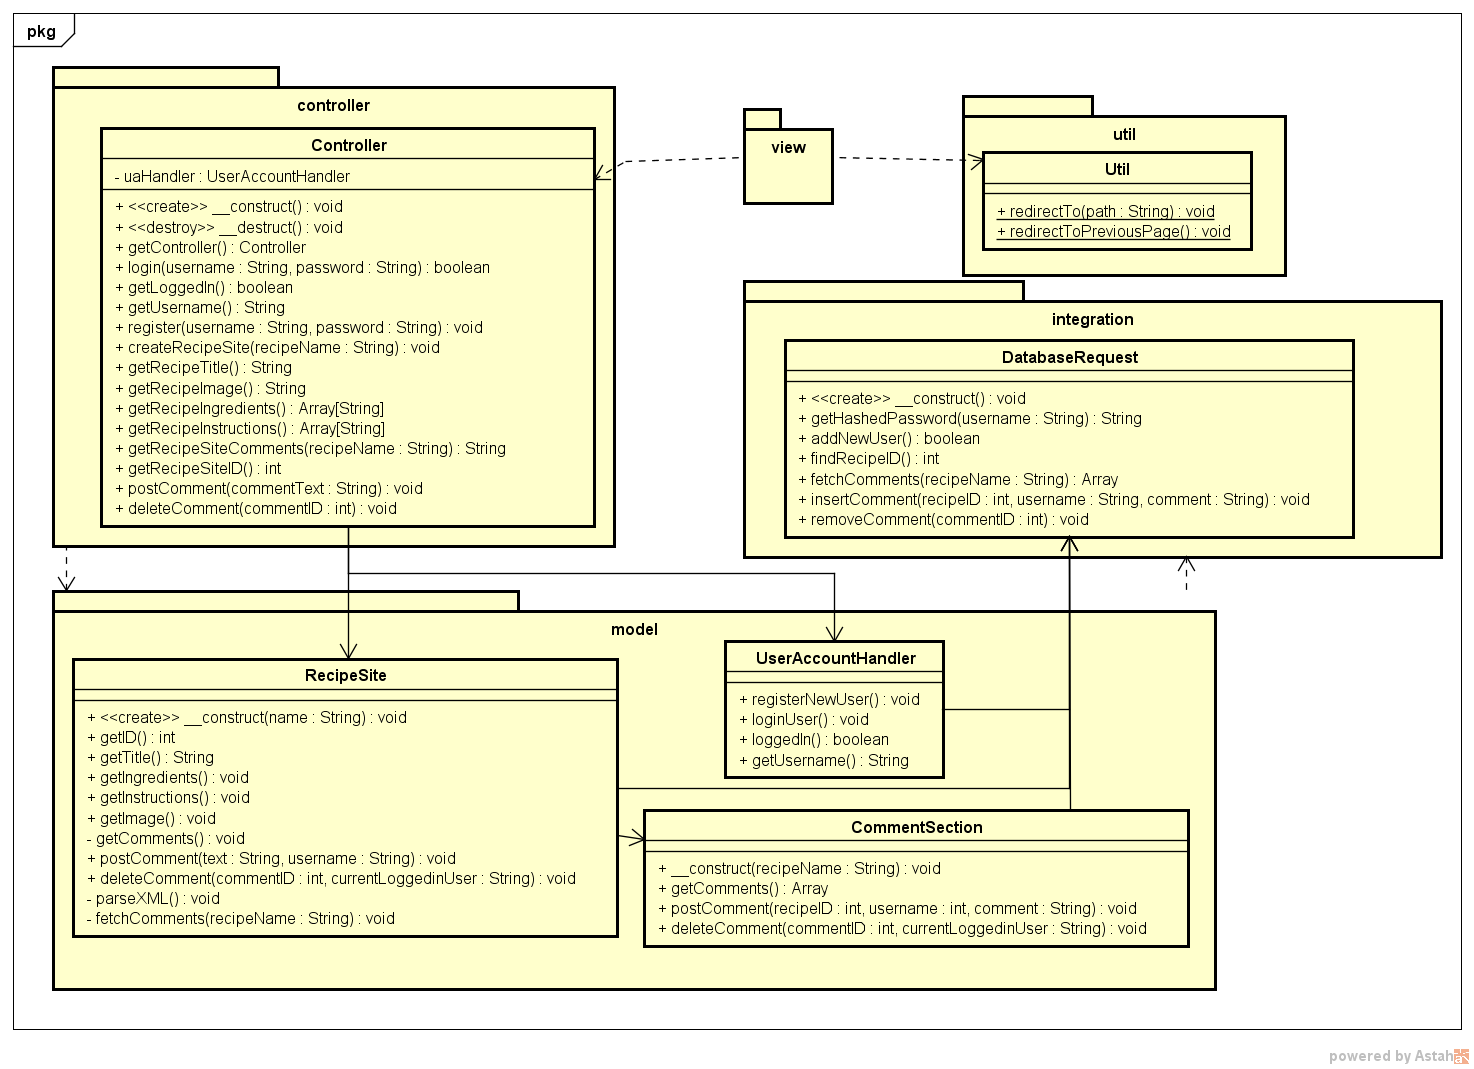
\includegraphics[scale=0.41]{img/TastyRecipesMVC.png}
    \caption{A class diagram describing the Tasty Recipes web application}
    \label{fig:classdia}
  \end{center}
\end{figure}

\section{Task 2}
I do not use HTTPS but HTTPS should be used whenever HTTP requests are being made by an authenticated user such as logging in, registering, or posting or deleting comments.

The file security of the system is strong on the webserver, as seen in Figure \ref{fig:ownership} and Figure \ref{fig:reqaccess}.

\begin{figure}[h!]
  \begin{center}
    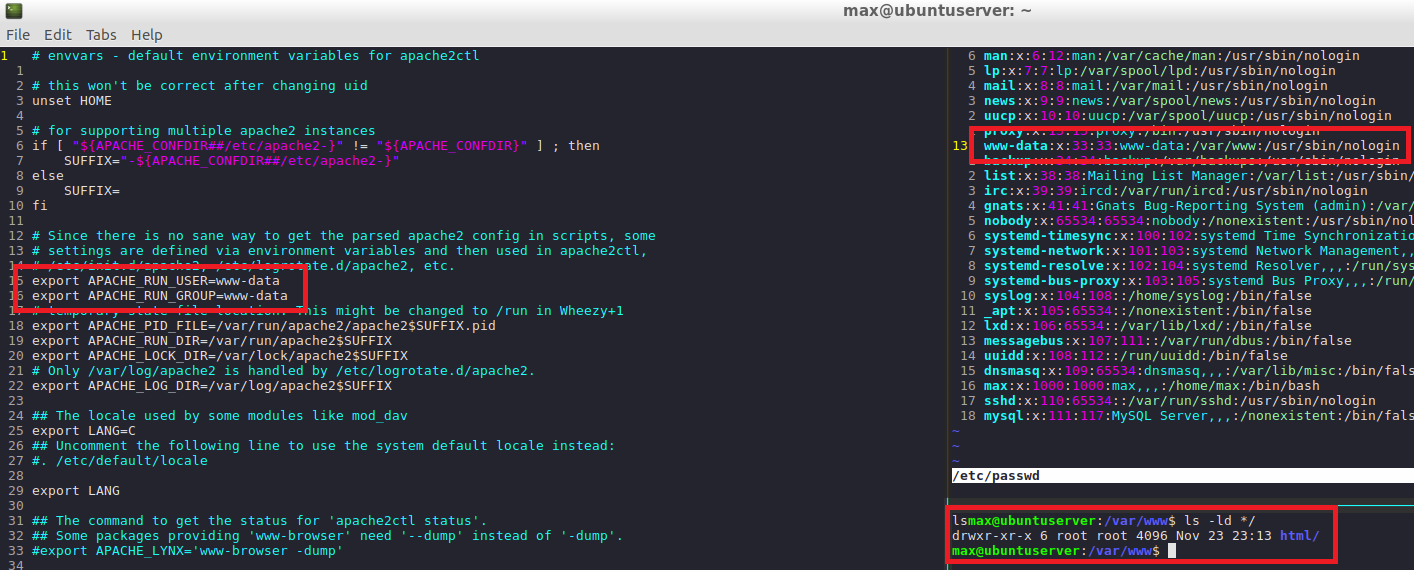
\includegraphics[scale=0.41]{img/filesecurity_ownership.png}
    \caption{Files showing apache username and web root file access.}
    \label{fig:ownership}
  \end{center}
\end{figure}

\begin{figure}[h!]
  \begin{center}
    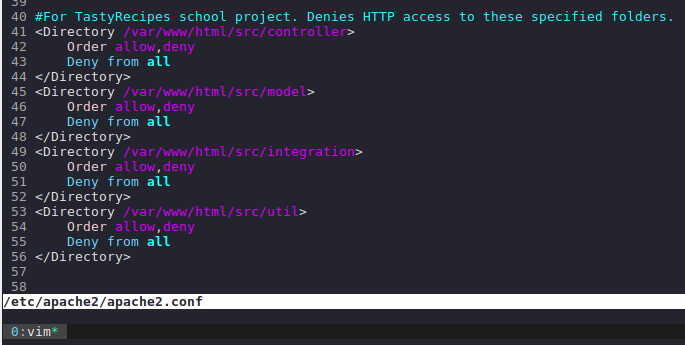
\includegraphics[scale=0.41]{img/filesecurity_reqaccess.png}
    \caption{The apache2 config file restricting HTTP access to all layers except the view}
    \label{fig:reqaccess}
  \end{center}
\end{figure}

Database security is maintained on the mySQL server using a unique user for the webapp, and by using parameterized queries in all requests to the database, as seen in \href{https://github.com/fongie/TastyRecipes/blob/assignment3/src/integration/DatabaseRequest.php}{this class file}.

Usage of password encryption can be seen \href{https://github.com/fongie/TastyRecipes/blob/86f4548c3b4659b762134c756cc5ac4c0cbf72a2/src/model/UserAccountHandler.php#L35}{here} and \href{https://github.com/fongie/TastyRecipes/blob/86f4548c3b4659b762134c756cc5ac4c0cbf72a2/src/model/UserAccountHandler.php#L18}{here}.

\section{Optional Task 2}

Database requests are made using the PDO library and SQL queries. All requests are made using a new instance of the \code{DatabaseRequest} class. The easiest way to see how data is inserted and extracted is to see the code for that class, \href{https://github.com/fongie/TastyRecipes/blob/assignment3/src/integration/DatabaseRequest.php}{here}.

\chapter{Discussion}

Implementing the MVC architecture from completely unstructured code was a long process and not very easy at first, the result is however a clear impementation of the MVC architecture. It helped tremendously to plan ahead using a class diagram. There are some requests that are passed down quite a long way, for example through the \code{Controller}, through a \code{RecipeSite} all the way to a \code{CommentSection}, but this is to reduce coupling on the \code{Controller} which now only has dependencies on two classes. All layers are well encapsulated, since all calls are made from the top and downwards. The \code{Util} class could have been left out but redirecting pages was so frequent in the view that I wanted to make a class for it. Since there were not many classes and files in this webapp I decided not to use a class autoloader. It makes it easier to keep track of what is actually imported, perhaps keeping a likeness to Java. Each import is required once instead.

The security implementations were straightforward following the instructions in the lecture notes, there is not much to discuss about that.

\chapter{Comments About the Course}

I spent more than 40 hours on this assignment.
As predicted after the previous assignment, structuring the code was a lot of work, despite having done the Object Oriented Design course last semester.
Implementing security was easy, especially using a linux web server.

\end{document}
